
\documentclass[a4paper,12pt]{article}

\usepackage[top=2.5cm, bottom=2.5cm, left=3cm, right=3cm]{geometry}
\setlength{\parskip}{10pt}

%% Mandatory stuff
\usepackage[utf8]{inputenc}
\usepackage[T1]{fontenc}

%% Math package
\usepackage{amsmath}
\usepackage{amssymb}
\usepackage{amsfonts}
\usepackage{mathrsfs}
\DeclareMathAlphabet{\mathpzc}{OT1}{pzc}{m}{it}

%Advanced tabular managers
\usepackage{array}
\usepackage{multirow}

% Improve itemize environment
\usepackage{enumitem}
\setlist[itemize]{noitemsep, topsep=0pt}% Delete useless space

%Figure managers
\usepackage{graphicx}
\usepackage{float}

%% Color package (for links, source code,...)
\usepackage[usenames]{color}
	%% Color for hyperlinks
\definecolor{colHyperlinks}{RGB}{0,90,170}%{59,0,159}

%% Hyperlinks for references (must be the last package loaded)
\usepackage[pdftex,%
  colorlinks,%
  linkcolor=colHyperlinks,%
  urlcolor=colHyperlinks,%
  citecolor=colHyperlinks,
  plainpages=false]{hyperref}
\begin{document}

\begin{center}
\Large{Licence L2\\Mathématiques pour l'informatique \\Contrôle Continu (30min)\\ 23 Septembre 2014}
\end{center}

\section*{Exercice 1}
On considère un ensemble $E = \mathbb{N}$, et une relation R sur E définie par :

\begin{center}
	$xRy \Leftrightarrow \exists p, q$ tel que $p\geq 1$ et $q \geq 1$, $y = px^q$ (avec $p, q \in \mathbb{N}$)
\end{center}

1) Tout en rappelant la définition de ces termes, vous montrerez si R est réflexive, symétrique, antisymétrique, transitive.

\begin{itemize}
	\item Réflexivité : R est réflexive si et seulement si $\forall x \in E,~ xRx$. On considère $p = q = 1$. On a bien $\forall x \in \mathbb{N},~ xRx$. Donc R est réflexive.
	\item Symétrie : R est symétrique si et seulement si $\forall x,y \in E,~ xRy \Rightarrow yRx$. On considère $2R4$ mais on s'aperçoit que nous n'avons pas $4R2$. Donc R n'est pas symétrique.
	\item Anti-symétrie : R est anti-symétrique si et seulement si $\forall x,y \in E, xRy \text{ et } yRx \Rightarrow x = y$. Si on a $xRy$ et $yRy$, alors on a $x\leq y$ et $y\leq x$. Ainsi, on a bien $x = y$. Donc R est anti-symétrique.
	\item Transitivité : R est transitive si et seulement si $\forall x,y,z \in E,~ xRy \text{ et } yRz \Rightarrow xRz$. Soit $xRy$ et $yRz$. Ainsi, $\exists p,q,a,b \geq 1$ tel que :
	$$y=px^q \text{ et } z = ay^b$$
	On en déduit :
	$$z = a(px^q)^b = (ap^b)x^{bq}$$
	Donc on a $xRz$ et R est bien transitive.
\end{itemize}

2) Après avoir rappelé ce qu'est une relation d'équivalence, vous direz si R est une telle relation.

R est une relation d'équivalence si et seulement si R est réflexive, symétrique et transitive. On a montré que R n'était pas symétrique. Ainsi, R n'est pas une relation d'équivalence.

3) Même question pour le cas d'une relation d'ordre.

R est une relation d'ordre si et seulement si R est réflexive, anti-symétrique et transitive. On a montré que ces propriétés sont vrais. Donc R est bien une relation d'ordre. 

\section*{Exercice 2}

Soit un ensemble $F = \{ \text{Alan}, \text{Bill}, \text{Charles}, \text{Donald}, \text{Edsger} \}$. On considère la relation d'ordre R sur F définie par les couples suivant :

$(\text{Alan}, \text{Alan})$, $(\text{Alan}, \text{Bill})$, $(\text{Alan}, \text{Charles})$, $(\text{Alan}, \text{Donald})$, $(\text{Alan}, \text{Edsger})$, $(\text{Bill}, \text{Bill})$, $(\text{Bill}, \text{Charles})$, $(\text{Charles}, \text{Charles})$, $(\text{Donald}, \text{Donald})$, $(\text{Donald}, \text{Charles})$, $(\text{Edsger}, \text{Bill})$, $(\text{Edsger}, \text{Charles})$, $(\text{Edsger}, \text{Donald})$, $(\text{Edsger}, \text{Edsger})$


1) Donner la matrice booléenne $M_R$ associée à R.

$$M_R = \left( \begin{array}{ccccc}
1&1&1&1&1\\
0&1&1&0&0\\
0&0&1&0&0\\
0&0&1&1&0\\
0&1&1&1&1
\end{array}\right)
$$

2) En déduire le graphe orienté $\mathpzc{G}_R$ de cette relation R (vous pourrez utiliser les initiales des prénoms).

\begin{figure}[hr!]
  \centering
    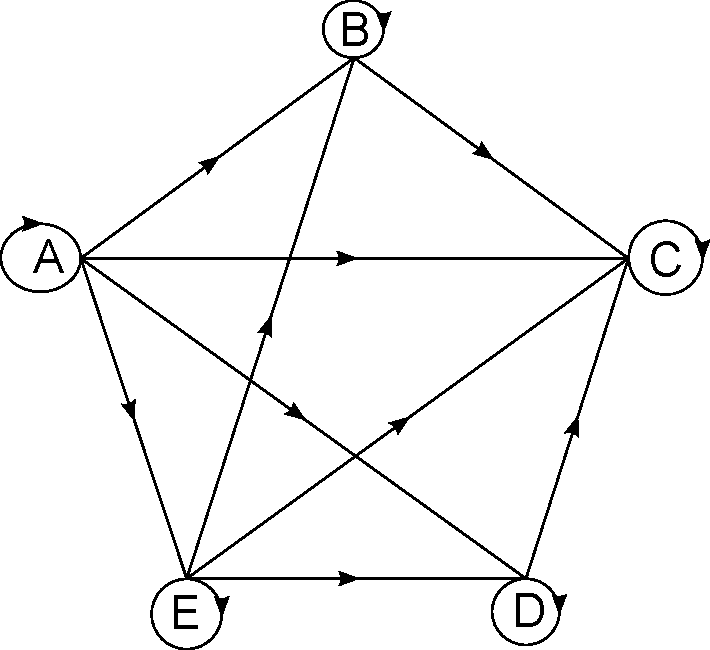
\includegraphics[width=.5\linewidth]{./exo2-graphe.pdf}
\end{figure}


3) Construire la diagramme de Hasse $\mathpzc{D}_R$ associé.

\begin{figure}[hr!]
  \centering
    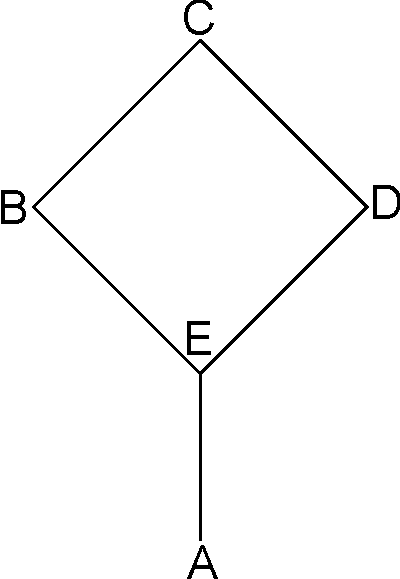
\includegraphics[width=.15\linewidth]{./exo2-hasse.pdf}
\end{figure}

% Alan Turing = créateur du premier calculateur électronique
% Bill Gates = Windows/Microsoft
% Charles Babbage = Conception de la première machine à calculer mécanique
% Donald Knuth = personne influente dans le monde de la programmation et père du TeX
% Edsger Dijkstra = personne influente dans le monde de l'informatique, et également connu pour son algorithme éponyme.

\end{document}